\chapter{Methodology}\label{c:method}
% \thispagestyle{fancy}


\section{Choice of Network architecture}

The field of \acp{SNN} is under ongoing research. Therefore many different network models and learning approaches have been proposed e.g. \acp{LSM}, REACH\cite{dewolf_spiking_2016}. To follow the idea that every spike contains information, purely rate based spiking networks are ignored as there is evidence that the precise spike timing is relevant in nature\cite{brette_philosophy_2015,putney_precise_2019}.\\

On the other side the use of \ac{HH}'s model is prohibitively complex. Additionally there are no training/learning rules available to solve such a high level problem.\\
The choice of Efficient coding networks allows us to retain all most of our biologic plausibility requirements while allowing the use of high level learning rules suited to our problem. Since the aim is to learn system dynamics, the \ac{SNN} should mirror this by learning the dynamics instead of a decoder in \acp{LSM}. Moreover the choice of Balanced networks enables us to potentially learn the decoder in addition to the dynamics as well. Lastly, with the proved properties towards noise and robustness it is optimally suited for our problem.
\section{Approach}
The construction of our \ac{SNN} can be separated into several blocks. Firstly, a \ac{SNN} is created for the simulation of a dynamic system with given external inputs.\\
As a second stage, we derive another \ac{SNN} that acts as the controller, delivering the relevant control signals to the first network.\\
With the controller in place, we work on learning the dynamics of the first \ac{SNN} from the ground up. Unfortunately, it was not possible to learn the dynamics of the controlling \ac{SNN}. However it is possible to avoid using a dedicated \ac{SNN} to act as a controller. By copying the key controlling behaviour of the control network we are able to control the trained network directly.\\
\section{Simulation of Dynamic systems using \acp{SNN}}\label{sec:simulation}
In the following sections the simulation of dynamic systems using \acp{SNN} is derived and explained. This serves as the a basic building block for the attempted method on how to solve our target set out in \cref{sec:goal}. We begin with the formal derivation of the network dynamics.

\subsection{Balanced network simulation}\label{ssec:balanced_network_sim}
This section follows the derivation found in \cite{boerlin_predictive_2013} and \cite{huang_dynamics_2019}.
The goal is to describe a dynamical system of the form
\begin{equation}\label{eq:x}
\bmu{\dot{x}} = \bmu{Ax} + \bmu{c}(t)
\end{equation}
with $J$ state variables.
The estimation is done by leaky integration of spike trains $\symbfup{o}(t)$ in
\begin{equation}\label{eq:x_hat}
\bmu{\dot{\hat{x}}} = -\lambda_d \bmu{\hat{x}} + \symbfup{\Gamma} \bmu{o}(t).
\end{equation}
$\bmu{\Gamma}$ is a given matrix of size $\mathbb{R}^{J\times N}$, $N$ being the number of neurons and given. $\bmu{o}(t)$ is the spike train of all neurons, specifically
\begin{equation}
	o_i(t) = \sum_k \delta(t - t^k_i)
\end{equation}
for neuron i with spike times at times $t_i^k$.\\
From \cref{eq:x_hat} it becomes clear that each spike carries an important information for the state vector as each spike in $\bmu{o}(t)$ changes the approximation $\bmu{\hat{x}}$ by some weights of $\bmu{\Gamma}$.
In addition to the estimate $\bmu{\hat{x}}$ we define a spiking rate variable $\bmu{r}$ following the dynamics of
\begin{equation}\label{eq:rate}
\bmu{\dot{r}} = -\lambda_d\bmu{r} + \bmu{o}(t).
\end{equation}
The rate variable is connected to the state vector in the decoding with
\begin{equation}\label{eq:decoding}
	\bmu{\hat{x}} = \bmu{\Gamma r}.
\end{equation}
The spiking dynamics arise from the minimization of a cost function. A spike is fired if it minimizes the cost function that tracks the error between the true and estimated value over time
\begin{equation}\label{eq:cost_func_basic}
E(t)=\int_0^t \|\symbfup{x}(u)-\hat{\symbfup{x}}(u)\|_2^2 \ du.
\end{equation}


\subsection{Greedy optimization of the cost}
The cost function \cref{eq:cost_func_basic} is minimized using a greedy optimization i.e. a spike is fired if it reduces the cost. For the derivation we use the cost function \cref{eq:cost_func} which is identical to setting $\mu = 0,\nu= 0$.\\
We express this as
\begin{equation}\label{eq:spike_condition}
	E(t|i \text{ spike}) < E(t,i \text{ }\overline{\text{spike}})
\end{equation}

If there is no spike fired, the rate and estimated state variable in \cref{eq:x_hat} and \cref{eq:rate} respectively behave as
\begin{equation}\label{eq:no_spike_decay}
\begin{aligned}
\bmu{\dot{\hat{x}}} &= -\lambda_d \bmu{\hat{x}}\\
\bmu{\dot{r}} &= -\lambda_d\bmu{r}
\end{aligned}
\end{equation}
and therefore decay exponentially with $e^{-\lambda_d t}$.\\
If a spike is fired at time $t^k$, the inhomogeneous solution is found by variation of constants in \cref{eq:rate} to
\begin{equation}\label{eq:rate_inhomo}
\begin{aligned}
r_i^h &= c_i(t)e^{-\lambda_d t}\\
c_i'(t) e^{-\lambda_d t} - c_i(t)\lambda_d e^{-\lambda_d t}&= -\lambda_d c_i(t)e^{-\lambda_d t} + \delta(t- t^k)\\
c_i'(t) &= \delta(t- t^k) e^{\lambda_d t}\\
c_i(t) &=  e^{\lambda_d t^k} \bm{H}(t-t^k)\\
r_i &=e^{-\lambda_d t} + e^{-\lambda_d (t-t^k)} \bm{H}(t-t^k).
\end{aligned}
\end{equation}
The last equation is the identical the solution of \cref{eq:no_spike_decay} with the addition of a decaying exponential added at time $t_i^k$. $\bm{H}(t)$ denotes the Heaviside step function. Analogously the estimate is updated at time $t^k$ to
\begin{equation}\label{eq:update_x_spike}
	\bmu{x} =  \bmu{x} + \bmu{\Gamma}_ie^{-\lambda_d (t-t^k)} \bm{H}(t-t^k).
\end{equation}
We look at the error a $\epsilon$ time in the future of $t^k$ and check \cref{eq:spike_condition}
\begin{equation}
\begin{aligned}
& \int_0^{t^k+\epsilon} \left(\underbrace{\left\|\bmu{x}(u)-\hat{\bmu{x}}(u)-\bmu{\Gamma}_i h(u-t^k)\right\|_2^2}_{\text{I}}+
\underbrace{\nu\left\|\bmu{r}(u)+\lambda_d \bmu{e}_i h(u-t^k)\right\|_1}_{\text{II}}\right.\\
& \left.+\underbrace{\mu\left\|\bmu{r}(u)+\lambda_d \bmu{e}_i h_d(u-t)\right\|_2^2}_{\text{III}}\right) d u\\
& <\int_0^{t^k+\epsilon} \left(\|\bmu{x}(u)-\hat{\bmu{x}}(u)\|_2^2+\nu\|\bmu{r}(u)\|_1+\mu\|\bmu{r}(u)\|_2^2\right)d u
\end{aligned}
\end{equation}
where we abbreviated $h(u) = e^{-\lambda_d (u)} \bm{H}(u)$.
To treat each term individually we start with I. Simplifying the norm we obtain
\begin{equation}
	\text{I} = \left\|\bmu{x}(u)-\hat{\bmu{x}}(u)\right\|_2^2 -2h(u-t^k)\bmu{\Gamma}_i^T\left(\bmu{x}(u)-\hat{\bmu{x}}(u)\right) + h^2(u-t^k)\bmu{\Gamma}_i^T\bmu{\Gamma}_i.
\end{equation}
For II the 1-norm and the rate holds that the $r_i(u)>0 \quad
\forall i$. Thus we can simplify $\|r\|_1 = \sum_k r_k$ resulting in
\begin{equation}
	\text{II} = \nu\left(\|r\|_1 + h(u-t^k)\right).
\end{equation}
Similarly to I, III can be simplified by $\|\bmu{r}\|^2_2 = \bmu{r}^T\bmu{r}$, giving
\begin{equation}
	\text{III} = \mu\|\bmu{r}\|^2_2 + \mu h^2(u-t^k) + 2\bmu{r}\cdot\bmu{e}_ih(u-t^k).
\end{equation}
After cancellation the remaining terms are grouped grouped by time dependency to yield
\begin{equation}
\begin{aligned}
	&\int_0^{t^k+\epsilon}h(u-t^k)\bmu{\Gamma}_i^T\left(\bmu{x}(u)-\hat{\bmu{x}}(u)\right) - \mu r_i(u) d u \\
	&> \frac{1}{2} \int_0^{t^k+\epsilon} 	h^2(u-t^k)\bmu{\Gamma}_i^T\bmu{\Gamma}_i + 	\nu h(u-t^k) + \mu h^2(u-t^k) d u
\end{aligned}
\end{equation}
Using the fact that the Heaviside function in \cref{eq:rate_inhomo} and subsequently in $h(u)$ allow us to change the borders of integration to $\int_{t^k}^{t^k+\epsilon}$. Lastly we simplify $h(t) = 1$ if $t\approx \epsilon$ and have
\begin{equation}
	\bmu{\Gamma}_i^T\left(\bmu{x}-\hat{\bmu{x}}\right) - \mu r_i>\frac{\|\bmu{\Gamma}\|^2 + \nu + \mu}{2}
\end{equation}
We notate the \ac{LHS} as the voltage

\begin{equation}\label{eq:voltage}
V_i(t)=\bmu{\Gamma}^T(\bmu{x}(t)-\hat{\bmu{x}}(t))-\mu r_i(t)
\quad i  = 1\dots N.
\end{equation}
and the constant \ac{RHS} as the voltage threshold $T_i$
\begin{equation}\label{eq:condition}
V_i>T_i=\frac{\left\|\boldsymbol{\bmu{\Gamma}}_i\right\|^2 + \nu+\mu}{2}.
\end{equation}

The dynamic variable $\bmu{x}$ is tracked by firing spikes in when the defined "voltage" of a neuron surpasses its threshold.\\
For negligible quadratic cost $\mu$ the voltage can be understood as measure of the error projected on $\bmu{\Gamma}_i$.
\subsection{Neuron Voltage}
As mentioned above, a neuron spikes if it meets the condition \cref{eq:condition}. But so far it is unclear how neuron voltage evolves over time.
Denote $\bmu{L}$ the the left pseudo-inverse of $\bmu{\Gamma}$
\begin{equation}
\bmu{L} = \left(\bmu{\Gamma}\bmu{\Gamma}^T\right)^{-1}\bmu{\Gamma}
\end{equation}
such that $\bmu{L}\bmu{\Gamma}^T = \bmu{I}$.\\
Next, taking the derivative of \cref{eq:voltage} yielding
\begin{equation}\label{eq:voltage_dt}
\bmu{\dot{V}}(t)=\bmu{\Gamma}^T\left(\bmu{\dot{x}}(t)-\dot{\hat{\bmu{x}}}(t)\right)-\mu \bmu{\dot{r}}(t).
\end{equation}
Now using the pseudo-inverse to rewrite the voltage equation \cref{eq:voltage} as
\begin{equation}\label{eq:voltage_2}
\begin{aligned}
\bmu{V}(t)&=\bmu{\Gamma}^T(\bmu{\hat{x}}(t)-\bmu{x}(t))-\mu \bmu{r}(t)\\
\bmu{L}\bmu{V}(t)&=(\bmu{x}(t)-\hat{\bmu{x}}(t))-\mu \bmu{L}\bmu{r}(t)\\
\bmu{x}(t)&=\bmu{L}\bmu{V}(t)  + \hat{\bmu{x}}(t) + \mu \bmu{L}\bmu{r}(t)\\
\end{aligned}
\end{equation}
Now the derivative terms in \cref{eq:voltage_dt} are replaced with  with their respective equations \cref{eq:x}, \cref{eq:x_hat} and \cref{eq:rate}. Lastly we substitute \cref{eq:voltage_2} in \cref{eq:voltage_dt} and obtain
\begin{equation}\label{eq:voltage_limit}
\begin{aligned}
	\bmu{\dot{V}} &= \bmu{\Gamma}^T\bmu{ALV}\\
	 &+ \left(\bmu{\Gamma}^T\bmu{A\Gamma} + \mu\bmu{\Gamma}^T \bmu{AL}+\lambda_d\bmu{\Gamma}^T\bmu{\Gamma} + \mu\lambda_d\right)\bmu{r}\\
	 &+\left(\bmu{\Gamma}^T\bmu{\Gamma} + \mu\bmu{I}\right)\bmu{o} + \bmu{\Gamma}^T\bmu{c}.
\end{aligned}
\end{equation}
The last argument is to consider the network behaviour for larger networks. We increase the number of neurons $N\longrightarrow\infty$ and require that the network output as well as the firing rates remains constant.\\
When looking at the decoding at \cref{eq:decoding} we therefore need to scale $\bmu{\Gamma}$ by $\frac{1}{N}$. To make sure that the threshold in \cref{eq:condition} will not get dominated by cost terms $\mu$ \& $\nu$, they should also scale with $\frac{1}{N^2}$. As the threshold decreases with $\frac{1}{N^2}$ so does the Voltage itself.\\
With this in mind, all terms that scale with $\frac{1}{N^2}$ are neglected. As a substitute for the neglected voltage term, a generic leak term is added making these \acp{LIF} neurons. The dynamics are therefore
\begin{equation}\label{eq:simple_sim}
\begin{aligned}
	\bmu{\dot{V}} &= -\lambda_V \bmu{V} + \bmu{W^sr} + \bmu{W^fo} + \bmu{\Gamma}^T \bmu{c} + \sigma_V\bmu{\eta}(t)\\
	\bmu{W^s} &= \bmu{\Gamma}^T\bmu{(A+\lambda}_d\bmu{I)\Gamma}\\
	\bmu{W^f} & = -\left(\bmu{\Gamma}^T\bmu{\Gamma} + \mu\bmu{I}\right)
\end{aligned}
\end{equation}

Lastly, to complete the derivation, a noise term $\bmu{\eta}$ with scaling factor $\sigma_V$ was added to simulate the inherent noise found in the brain.

\subsection{Regularization}\label{sssection:regularization}

Two regularization terms were added to influence spiking behaviour.

\begin{equation}\label{eq:cost_func}
E(t)=\int_0^t \left(\|\symbfup{x}(u)-\hat{\symbfup{x}}(u)\|_2^2+\nu\|\symbfup{r}(u)\|_1+\mu\|\symbfup{r}(u)\|_2^2\right)d u
\end{equation}

The parameter $\nu$ controls the amount of spiking by penalizing the total number of spikes as
\begin{equation}
||r(t)||_1 = \sum_i|r_i(t)| = \sum_i r_i(t).
\end{equation}
The firing rate is directly related to the number of spiking and therefore the cost is reduced by fewer spikes.\\

The second term solves different issues at the same time. One problem concerns networks that have decoding kernels with the same direction but opposite sign. To show this we imagine a network of only two neurons. A network of two neurons is sufficient to simulate a scalar \ac{ODE} i.e $\bmu{A}\in \mathbb{R}$. We further assume that the feed-forward weights $\bmu{\Gamma}$ has the form
\begin{equation}
\Gamma = \begin{bmatrix}
-1\\1
\end{bmatrix}
\end{equation}
Ignoring the cost terms in \cref{eq:condition} the threshold is set at
\begin{equation}
V_i > \frac{\|\bmu{\Gamma}_i\|^2}{2}
\end{equation}
after which that a spike is fired and the voltage of neuron $i$  resets to
\begin{equation}
V_i = V_i + \bmu{W^s}_{ii} = V_i + \|\bmu{\Gamma}_i\|^2_2 \quad \text{ with } \bmu{W^f} = \begin{bmatrix}
-1& 1\\
1& -1
\end{bmatrix}
\end{equation}
ideally setting the Voltage to $-T_i$. This can be seen when looking at the threshold as
\begin{equation}
T_i =\frac{ \bmu{\|\Gamma}_i\|^2}{2}= \frac{-\text{diag}(\bmu{W^f})}{2}.
\end{equation}
The repolarization of the spiking neuron acts as a depolarization or pushing the voltage towards its threshold for neurons with opposing sign. The problem now is that for neurons with the same kernel magnitude the depolarization is larger enough to push this neuron over the threshold. The subsequent spike re-polarizes the neuron but in turn excites the first neuron over its threshold. This back and forth pattern of "ping-ponging" repeats indefinitely.\\
For the given example above, the threshold is given by 0.5 for both. The neurons' voltages of are identical up to the sign, since they are tracking the error for the same variable. At the time one neurons reaches the threshold of 0.5 the second neuron's voltage is close to -0.5 considering noise (in a perfect system minus the value of the spiking neuron). After the spike is fired, the first neuron is reset to -0.5 stemming from
\begin{equation}\label{eq:reset}
\begin{aligned}
\bmu{V} &= \bmu{V} + \bmu{W^fo} = \bmu{V} + \bmu{W^f}\begin{bmatrix}
1\\
0
\end{bmatrix} = \bmu{V} + \bmu{W^f}_{:0}\\
\bmu{V} &= \begin{bmatrix}
0.5\\
-0.5\\
\end{bmatrix} +
\begin{bmatrix}
-1\\
1\\
\end{bmatrix} =
\begin{bmatrix}
-0.5\\
0.5
\end{bmatrix}
\end{aligned}
\end{equation}
$\bmu{W^f}_{00}$ whereas the second neuron gets pushed up to 0.5 , causing a spike. This in turn reverts the changes of \cref{eq:reset} resulting in a loop. This problem is caused by the greedy optimization, looking only at the immediate future to decrease the cost.\\
To fix this the threshold is slightly increased, disallowing a spike to reach the opposing neuron's threshold. As seen above in \cref{eq:condition}, this can be done by either raising the linear or quadratic cost.\\
The second issue fixed by adding quadratic cost is when there are
neurons with similar kernel direction but non normalized. In a perfect noise free scenario the neuron with the smaller threshold will always fire first. The neurons reset after the spike will reset the neurons with similar direction, inhibiting the second neuron from ever firing. The linear cost does not make a difference since it is penalizing the global number of spikes but does not discern where the neurons are firing. By penalizing the rate in the 2-norm it forces the network to spread the firing among the whole network.


\section{Control of Dynamic systems using \acp{SNN}}\label{sec:control}
\subsection{Balanced networks as a controller}
We now make the step to use the balanced network approach from above as a controller mechanism.\\
The idea was adopted from \cite{huang_optimizing_2017} and is illustrated in \cref{fig:schematic}. With the given reference signal, the produced network spikes are decoded into a control signal which is then further fed into the dynamical system.\\
The system itself is simulated using a common numerical method i.e. explicit Euler. Yet the goal is to capture the entire problem using \acp{SNN}. The control signal $\bmu{u}$ is generated using the an independent \ac{SNN} which is in turn the command $c$ for a separate \ac{SNN} simulating the states with feedback to the controlling \ac{SNN}.
\begin{figure}
	\centering
	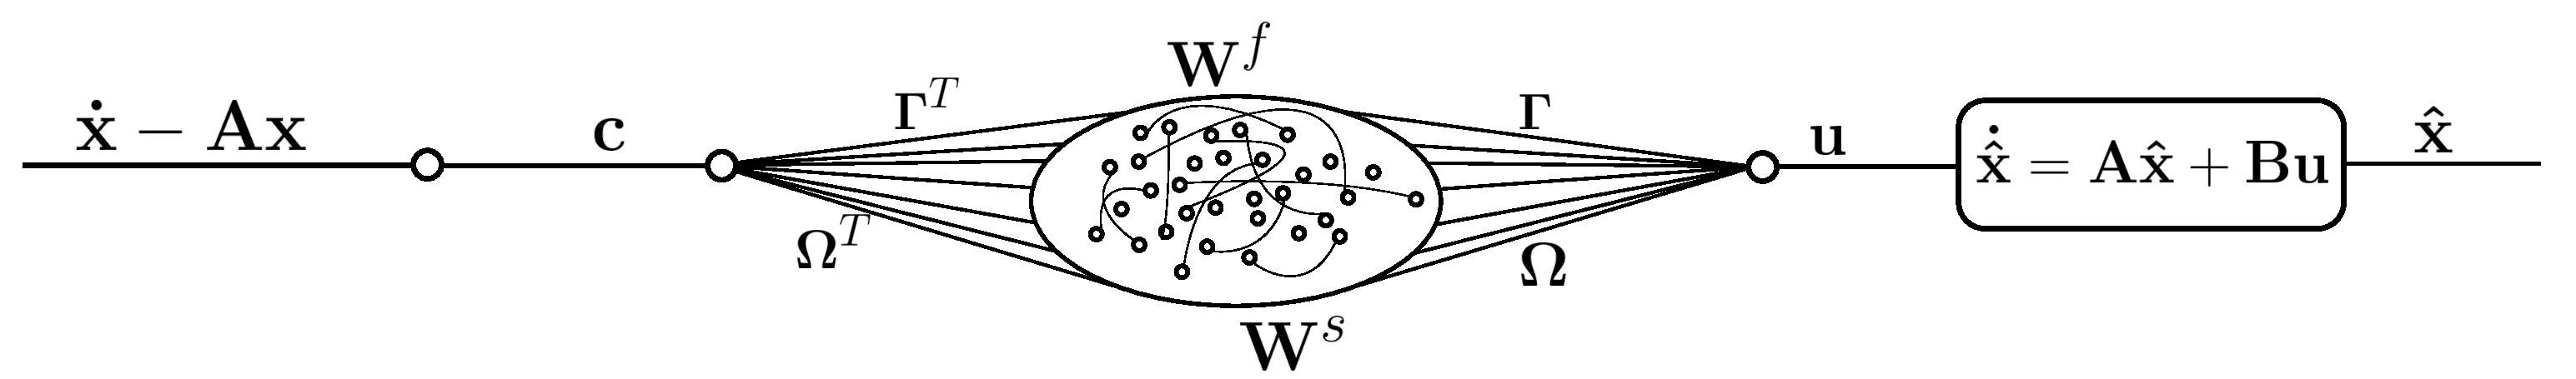
\includegraphics[width=\textwidth]{svg-inkscape/schematic_controller_network.pdf}
	\caption{Schematic to illustrate the use of balanced networks as controllers.}
	\label{fig:schematic}
\end{figure}
\subsection{Dynamics}\label{ssec:control_dynamics}
The derivation of this method is similar to the one in \cref{sec:simulation}. Names and variables are reused if not stated here.\\
The system in question has the form
\begin{equation}\label{eq:contsys}
	\bmu{\dot{\hat{x}}} = \bmu{A\hat{x}} + \bmu{Bu}.
\end{equation}
The basic definitions of the \ac{SNN} remain the same with rate $\bmu{r}$ as well as decoding weights $\bmu{\Gamma}$. Additionally, \cite{huang_optimizing_2017} defines instantaneous decoding weights $\bmu{\Omega}$ with the same shape as $\bmu{\Gamma}\in \mathbb{R}^{J\times N}$. It is important to note that $J$ does not represent the number of state variables but the number of inputs. The decoding is the same as in \cref{eq:decoding} with the added $\bmu{\Omega}$ giving.
\begin{equation}\label{eq:control_signal_comp}
	\bmu{u}(t) = \bmu{\Gamma r} + \bmu{\Omega o}.
\end{equation}
The derivation of the network dynamics in \cite{huang_dynamics_2019} is similar to \cite{boerlin_predictive_2013} and the derivation presented above. Differences arise in the computation of the cost function as the spike changes the system to
\begin{equation}\label{eq:control_spike_change}
	\begin{aligned}
	\bmu{u} &= \bmu{u} + h(t-t^k)\bmu{\Gamma}_k + \bmu{\Omega}_k\\
	\bmu{r} &= \bmu{r} + h(t-t^k)\bmu{e}_k\\
	\bmu{\hat{x}} &= \bmu{\hat{x}} + h(t-t^k)\int_{0}^{t-t^k}e^{(\bmu{A}+\lambda_d\bmu{I})\zeta}d\zeta \bmu{B\Gamma}_k + e^{A(t-t^k)}\bmu{B\Omega}_k
	\end{aligned}
\end{equation}
where $\bmu{\Gamma}_k$ and $\bmu{\Omega}_k$ correspond to the $k$-th column of $\bmu{\Gamma}$, $\bmu{\Omega}$ and $h$ the same as defined above. Results are similar for the rate and control signal whereas the state update is obtained by formally integrating the system. The rest of the derivations are analogous and completely derived in \cite{huang_optimizing_2017}. The results summarize to \crefrange{eq:control_dyn_begin}{eq:control_dyn_end}.
\begin{align}
	\bmu{V} &= \bmu{\Omega}^T\bmu{B}^T\left(\bmu{x} -\bmu{\hat{x}}\right) - \mu \bmu{r}\label{eq:control_dyn_begin}\\
	\bmu{\dot{V}} &= -\lambda_V\bmu{V} + \bmu{\Omega}^T \bmu{B}^T \bmu{c}(t) + \bmu{W^fo} + \bmu{W^sr}\label{eq:control_dyn_2}\\
	\bmu{c} &= \bmu{\dot{x}} - \bmu{Ax}\\\label{eq:feeback_c}
	\bmu{W^f} &= - \left(\bmu{\Omega}^T\bmu{B}^T\bmu{B\Omega} + \mu\bmu{I}\right)\\
	\bmu{W^s} &= -\bmu{\Omega}^T\bmu{B}^T\bmu{B\Gamma}\label{eq:Ws_wrong}\\
	T_i &= \frac{\bmu{\Omega}_i^T\bmu{B}^T\bmu{B\Omega}_i + \nu  + \mu}{2}
	\label{eq:control_dyn_end}
\end{align}
Note that the notation differs in the original paper and the reference signal is denoted by $\bmu{\hat{x}}$ instead of $\bmu{x}$ here and $\bmu{\Omega}_i$ again refers to the $i$-th column of $\bmu{\Omega}$.
\subsection{The instantaneous decoding weights}
The presence of instantaneous decoding is necessary otherwise no spiking can occur. In \cref{eq:control_spike_change} the control signal is integrated with the matrix exponential. The problem is that the integral
\begin{equation}
	\lim_{t\longrightarrow 0 } \int_0^t e^{(\bmu{A}+\lambda_d\bmu{I})\zeta}d\zeta = 0
\end{equation}
for our small $\epsilon$ time horizon.\\
This is true for any matrix exponential $e^{\bmu{\Lambda}\zeta}$ seen by Taylor expansion
\begin{equation}
	\begin{aligned}
	\lim_{t\longrightarrow 0 }\int_0^t e^{\bmu{\Lambda}\zeta}d\zeta &= \lim_{t\longrightarrow 0 } \int_0^t \sum_{k=0}^\infty \frac{\left(\bmu{\Lambda}\zeta\right)^k}{k!} d\zeta\\
	&=\lim_{t\longrightarrow 0 }\sum_{k=1}^\infty t\frac{\left(\bmu{\Lambda}t\right)^{k-1}}{k!} = 0.
	\end{aligned}
\end{equation}
This means that the rate decoding vanishes in the derivation of \crefrange{eq:control_dyn_begin}{eq:control_dyn_end}. Therefore the firing threshold condition becomes
\begin{equation}
	-\mu \bmu{r}_i > \frac{\nu  + \mu}{2}
\end{equation}
if $\bmu{\Omega}$ is ignored which is an insatiable condition since $\bmu{r}$ is always non-negative.
\subsection{Extension with direct Error feedback}\label{ssec:extension}
The same group of \cite{huang_optimizing_2017} later published a new but very similar approach in \cite{huang_spiking_2019} which is based on the same idea, however the approach in \cite{huang_spiking_2019} makes the error a direct part of the voltage dynamics. The difference arises from the an new derivation avoiding the pseudo-inverse $\bmu{L}$.\\
Instead, during the analogous step of \cref{eq:voltage_dt} they set $\bmu{\hat{x}}$
and $\bmu{x}$ to follow the same dynamics, namely
\begin{equation}\label{eq:feedback_c2}
	\bmu{\dot{x}} = \bmu{Ax} + \bmu{c}(t)
\end{equation}
for the reference signal and
\begin{equation}
	\bmu{\dot{\hat{x}}} = \bmu{A\hat{x}} + \bmu{Bu}
\end{equation}
for the system.\\
In total this adjustment changes the dynamics of \cref{eq:control_dyn_2} to
\begin{equation}\label{eq:direct_error_voltage}
	\bmu{\dot{V}} = -\lambda_V\bmu{V} + \bmu{\Omega}^T \bmu{B}^T\bmu{Ae}(t) + \bmu{\Omega}^T \bmu{B}^T \bmu{c}(t) + \bmu{W^fo} + \bmu{W^sr}.
\end{equation}
Due to the assumption of \cref{eq:feedback_c2} the derivation changes in two aspects. Firstly, the construction of the pseudo-inverse can be avoided, making the consideration of the limit is rendered obsolete. Instead of eliminating the $\bmu{x}$ it is kept directly in the voltage equation and with the substitution of \cref{eq:feedback_c2}. Without considering the limit, the definition of $\bmu{W}^s$ changes to
\begin{equation}
	\bmu{W^s} = -\bmu{\Omega}^T\bmu{B}^T\bmu{B\Gamma} + \mu\bmu{I}.
\end{equation}
As done previously, a white noise process $\bmu{\eta}$ is added to complete the dynamics.
\section{Learning of network parameters}\label{sec:learning}
All the methods described above work on the optimally ideal weights for the dynamics. However in nature often new skills or dynamics are learned and not optimally tuned for the problem at hand. In the following chapter the optimally of derived is explained and local learning rules for the weights are introduced. Specifically, the learning rules presented in \cite{bourdoukan_learning_2012,brendel_learning_2020,bourdoukan_enforcing_2015}.


\subsection{Learning of fast connection weights $\bmu{W}^f$}
Before deriving the learning rule, we are first going to establish the idea that the minimization of the loss is equal to minimizing the fluctuations of the membrane potential.\\
This assumption is based on the fact that the Voltage is the projected error of the tracked signal to the reference. Therefore a good tracking should cancel out
\begin{equation}
	\bmu{V} = \bmu{\Gamma}\big(\bmu{x} - \bmu{\hat{x}}\big) \approx \bmu{0}
\end{equation}
neglecting the regularization terms.\\
Therefore, the average membrane voltage
\begin{equation}
	L = \int_0^T\|\frac{1}{2}\bmu{V}(t)\|^2dt
\end{equation}
over time serves as a good and simple measure of tracking performance.\\
Since the Voltage is bound by the threshold, the computation of the average can be reduced to averaging of the spikes.\\
\paragraph{Learning with $\bmu{L_1}$ costs}
As such, the minimal variation is given if the voltage threshold and its respective reset are centred around zero. Voltage resets, given by $\bmu{W}^f_i$ for spiking neuron $i$, need to be strengthened if its reset undershoots the negative threshold value $T_i$ and vice versa. A spiking reset that hyperpolarized the neuron over the negative threshold will be weakened.\\
Mathematically, this averaging over spikes condition is formulated as the loss at time $t$, using the fact we can express the Voltage post-spike $\bmu{V}^{\text {post}}$ as
\begin{equation}
	\bmu{V}^{\text {post}} = \bmu{V}^{\text {pre}} + \bmu{W}^f \bmu{e}_i
\end{equation}
for neuron $i$ firing a spike.\\
Taking the derivative of the loss function in \cref{eq:vol_bases_loss} with respect to $\bmu{\Omega}$ yields
\begin{equation}
\frac{\partial L_t}{\partial \bmu{W}^f} \propto\left(2 \bmu{V}^{\text {pre}}\left(t\right)+\bmu{W}^f \bmu{e}_{i}\right) \bmu{e}_{i}^{T}
\end{equation}
Rewriting the equation above and adding a tuning parameter gives the learning rule
\begin{equation}\label{eq:Wf_learning_rule_1}
	\Delta \bmu{W}^f_{ij} =-\frac{\partial L_t}{\partial \bmu{W}^f_{ij}} \propto - \left( \bmu{V}_i^{\text {pre}}\left(t\right)+\beta \bmu{W}^f_{ij}\right).
\end{equation}
It is important to note that this learning rule only becomes active during the firing of a spike. This means that if no spike is fired no learning takes place. To introduce spiking and learning, smoothed  Gaussian white noise if often used for training and inducing firing of all neurons.\\
The role of $\beta$ is to regulate the amount of spiking by artificially increasing the magnitude of the recurrent weights. Therefore, with increased magnitude neurons are overly hyperpolarized after a spike making it harder to spike again soon, similar how the linear costs above reduce spiking activity.\\
Choosing $\beta \approx \frac{1}{2}$ will lead to low linear costs at the risk of degrading into ping-ponging patterns described previously. It is important to note that this learning rule is entirely local and can be categorized as a Hebbian learning rule, as the presynaptic voltage is multiplied by the postsynaptic reset, given by the column in $\bmu{W}^f$.\\
\paragraph{Learning with $\bmu{L_2}$ costs}
The previous derivation did only incorporate $L1$ costs using the $\beta$ parameter, but does not implement any $L2$ regularization as in the derivation in \cref{sec:simulation}. With L2 costs, the optimal matrix is given by the addition of the quadratic cost term to the diagonal as in \cref{eq:simple_sim}. Since the cost term is added to the matrix $\bmu{W}^f$ and the voltage definition in \cref{eq:voltage} the voltage no longer explicitly tracks the projected error. To reuse the argument about minimizing Voltage fluctuations as a performance measure we therefore add the terms again to cancel out the terms from the previous definition. Specifically, we want to work the true projection error $\bmu{V}_{\text{ex}}$ and therefore compute the loss in \cref{eq:vol_bases_loss} using
\begin{equation}\label{eq:Wf_learning_rule_improved}
\begin{aligned}
	\bmu{V}_{\text{ex}} &= \bmu{V} + \mu\bmu{r}\\
	\bmu{W}^f_{\text{ex}} & = \bmu{W}^f + \mu\bmu{I}.
\end{aligned}
\end{equation}
We then formulate the same argument on the loss
\begin{equation}\label{eq:vol_bases_loss}
\begin{aligned}
L_t & =\left\|\frac{1}{2}\big(\bmu{V}^{\text {pre}}_{\text{ex}}\left(t\right)+\bmu{V}^{\text {post}}_\text{ex}\left(t\right)\big)\right\|^2 \\
& =\left\|\bmu{V}^{\text {pre}}\left(t\right)+ \mu\bmu{r}\left(t\right) + \frac{1}{2}\left(\bmu{W}^f + \mu \bmu{I}\right)\bmu{e}_{i}\right\|^2
\end{aligned}
\end{equation}
and take the derivative with respect to $\bmu{W}^f$, resulting in the learning rule of the form
\begin{equation}
\Delta \bmu{W}^f_{ij} =-\frac{\partial L_t}{\partial \bmu{W}^f_{ij}} \propto - \beta\left( \bmu{V}_i^{\text {pre}}\left(t\right) + \mu \bmu{r}_i(t)\right) -\bmu{W}^f_{ij} -\mu\delta_{ij}
\end{equation}
when a spike is fired.

\subsection{Learning of slow connection weights $\bmu{W}^s$}
The recurrent weights $\bmu{W}^s$ are called slow because they are in conjunction with the filtered spike train $\bmu{r}(t)$ in \cref{eq:voltage_limit} in contrast to $\bmu{W}^f$ which are reset the neuron voltage after a spike.\\
For learning $\bmu{W}^s$ an adaptive learning approach from \cite{bourdoukan_enforcing_2015} is used.\\
\begin{figure}[H]
	\centering
	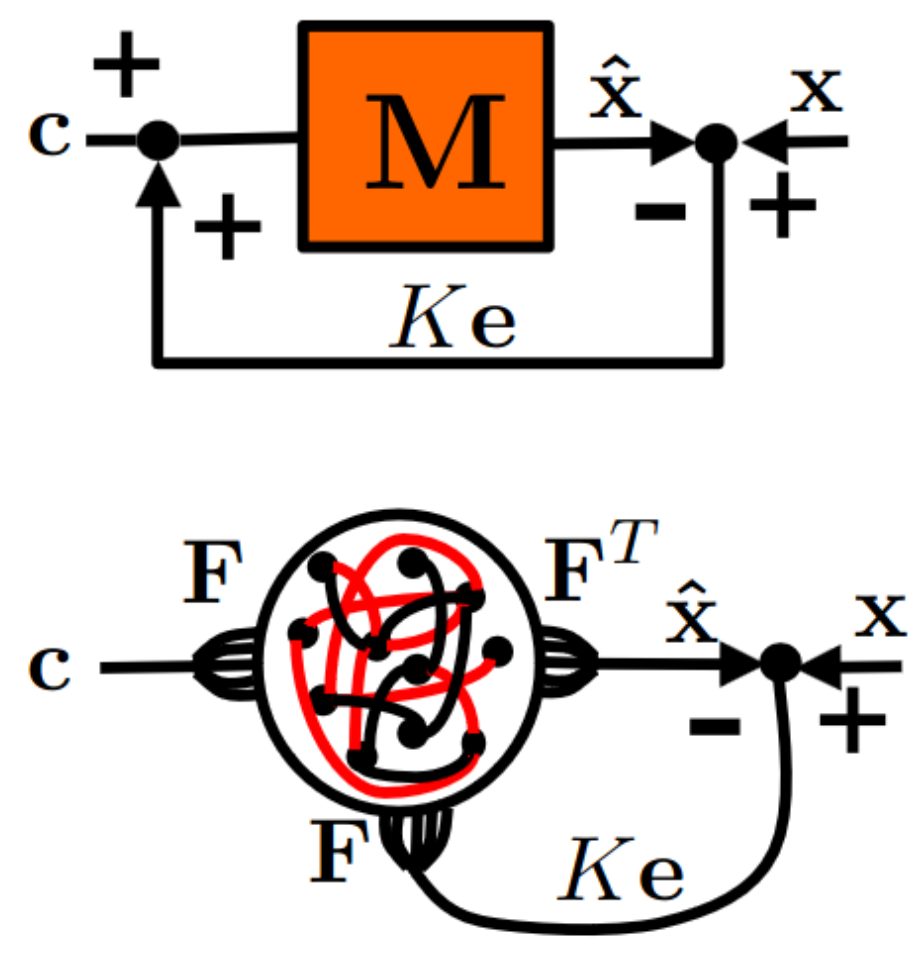
\includegraphics[scale = 0.15]{screenshots/error_feedback_Ws.png}
	\caption{Schematic of error feedback in the learning of $\bmu{M}$ resp. $\bmu{W}^s$. Taken from \cite{bourdoukan_enforcing_2015}.}
	\label{fig:error_feedback_Ws}
\end{figure}
For this we consider a "learner" dynamic system of the form
\begin{equation}
	\dot{\hat{\bmu{x}}} = \bmu{M}\hat{\bmu{x}} + \bmu{c}(t)
\end{equation}
where the matrix $\bmu{M}$ changes to allow $\hat{\bmu{x}}$ to follow the same dynamics of $\bmu{x}$ given by
\begin{equation}\label{eq:teacher}
	\bmu{\dot{x}} = \bmu{Ax} + \bmu{c}(t).
\end{equation}
Over time, $\bmu{M}$ should converge to $\bmu{A}$. To facilitate this, the error $\bmu{e} = \bmu{x} - \hat{\bmu{x}}$ is feed back into the learner system $\dot{\hat{\bmu{x}}} =\bmu{M}\hat{\bmu{x}} + \bmu{c}(t)  + K\bmu{e}$ to direct $\bmu{M}$.
The adjustment of $\bmu{M}$ in the modified dynamics
\begin{equation}\label{eq:student}
	\dot{\hat{\bmu{x}}} = \left(\bmu{M} + K\bmu{I}\right)\hat{\bmu{x}} + \bmu{c}(t) + K\bmu{x}
\end{equation}
is then calculated by using minimizing the loss
\begin{equation}
	L = \frac{1}{2}\bmu{e}^T\bmu{e}
\end{equation}
with respect to the matrix parameters $M_{ij}$ and changing their value according to
\begin{equation}\label{eq:learning_rule_Ws}
	\dot{M}_{ij} = -\frac{\partial L}{\partial M_{ij}} = \left(\frac{\partial \hat{\bmu{x}}}{\partial M_{ij}}\right)^T\bmu{e}.
\end{equation}
The derivative in $\frac{\partial \hat{\bmu{x}}}{\partial M_{ij}}$ is computed under the assumption that $K$ is much larger than the eigenvalues of $\bmu{M}$ and $\bmu{c} = const$. As a simplification we choose $\bmu{c} = \bmu{0}.$ and formerly integrate \cref{eq:teacher} to obtain $\bmu{x} = e^{\bmu{A}t}\bmu{x_0}$. We plug this in \cref{eq:student}, solve again and obtain
\begin{equation}\label{eq:hat_x_derivative}
	\hat{\bmu{x}} = \left(\bmu{A} + K\bmu{I} - \bmu{M}\right)^{-1}K e^{\bmu{A}t}\bmu{x_0} + e^{\left(\bmu{M}- K\bmu{I}\right)t}\hat{\bmu{x}}_{\bmu{0}}  \approx e^{\left(\bmu{M}- K\bmu{I}\right)t}\hat{\bmu{x}}_{\bmu{0}}.
\end{equation}
The first term is neglected due to the assumption and the inverse approximation
\begin{equation}
	\left(K\bmu{I} + \bmu{A} - \bmu{M}\right)^{-1}  = K^{-1}\bmu{I} - K^{-2}\left(\bmu{A} - \bmu{M}\right)^{-1} + \mathcal{O}(\|\bmu{A - \bmu{M}}\|^2).
\end{equation}
From this approximation the desired derivative of \cref{eq:learning_rule_Ws} is given by
\begin{equation}
	\frac{\partial L}{\partial \bmu{M}}\propto \hat{\bmu{x}}^T\bmu{e}
\end{equation}
To convert this learning rule for the system $\bmu{A}$ into a learning rule for the $\bmu{W}^s$ the change of $\bmu{W}^s$ is identified by a change in the underlying dynamical system $\bmu{\Gamma}^T \bmu{M \Gamma}$. The corresponding learning rule becomes
\begin{equation}
	\dot{\bmu{W}}^s \propto \bmu{\Gamma}\dot{\bmu{M}}\bmu{\Gamma}.
\end{equation}
Another interpretation of the formulation is in a form of feedback alignment. As the error is feed back into the network via $\bmu{\Gamma}$ (\cref{fig:error_feedback_Ws}), the matrix $\bmu{M}$(and in extension $\bmu{W}^s$) self-aligns to the error along $\bmu{\Gamma}^T$.
This has been demonstrated in \cite{lillicrap_random_2016} and has shown comparable performance to \ac{BP}.